\section{Шифр DES}\index{шифр!DES|(}
\selectlanguage{russian}

Развитием проекта <<Люцифер>>\index{шифр!Люцифер} стал государственный стандарт США, известный как DES (\langen{data encryption standard}). Это первый из рассматриваемых нами блочных шифров, который имеет ярко выраженные раунды шифрования, отдельно выделенную функцию ключевого расписания и основан на классической ячейке Фейстеля\index{ячейка Фейстеля}. Поэтому для знакомства с шифром достаточно рассмотреть устройство функции Фейстеля\index{функция!Фейстеля} как основного элемента, отличающего данный шифр от аналогичных.

В шифре DES открытый текст делится на блоки по 32 бита, и они обрабатываются в 16 раундах. Раундовые ключи генерируются из исходных 64 бит ключа (при этом значащими являются только 56 бит, а последние 8 бит используются для проверки корректности ввода ключа). На вход функции Фейстеля для шифра DES, схема которой приведена на рис.~\ref{fig:des}, подаётся половина от размера входного блока -- 32 бита.

\begin{figure}[!htb]
    \centering
    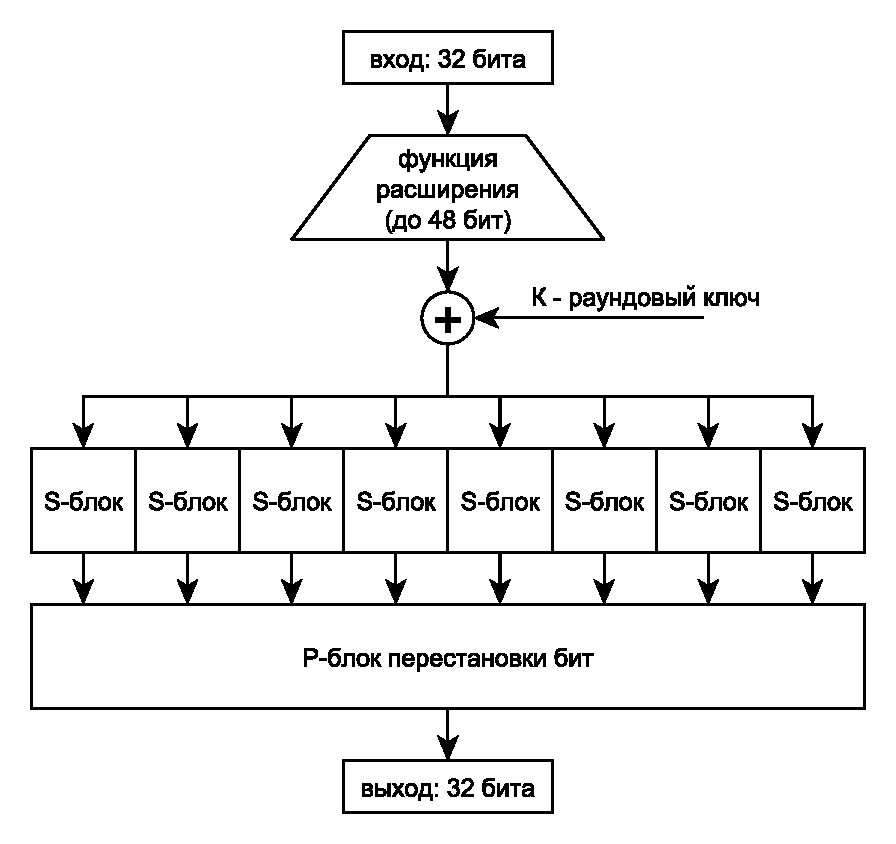
\includegraphics[width=0.75\textwidth]{pic/des}
    \caption{Функция Фейстеля\index{функция!Фейстеля} шифра DES\label{fig:des}}
\end{figure}

Эти 32 бита проходят через функцию расширения, которая с помощью дублирования отдельных битов превращает их в 48 бит. Они суммируются побитово по модулю 2 с раундовым ключом. Результат подаётся на вход 8 s-блоков, которые работают как таблицы замен последовательности из 6 бит в 4 бита (каждый блок). На выходе s-блоков получаются $8 \times 4 = 32$ бита, которые попадают в p-блок перестановки. Результат работы p-блока является результатом функции Фейстеля\index{функция!Фейстеля} для одного раунда шифра DES.

Интересно отметить, что изначально автором предполагалось использовать ключ в 128 бит, но под напором АНБ (Агентство национальной безопасности, \langen{National Security Agency, NSA}) он был сокращён до 56 бит, что на тот момент составляло вполне достаточную для криптостойкости величину. Кроме того, АНБ указало обязательные к использованию s-блоки (таблицы замен). Много позже, в 90-х годах, когда были разработаны методы линейного и дифференциального криптоанализа, выяснилось, что предложенные АНБ в 70-х годах s-блоки устойчивы к данным методам криптоанализа, как будто специально делались с учётом возможности их использования.

\index{шифр!DES|)}
